% New manuscript. Historical paper/PHASE_TTC_Final.tex is preserved.
% Build: python build_revision.py (from this directory).
\documentclass[twocolumn,letterpaper]{article}
\usepackage{phase_style}
\hypersetup{pdftitle={PHASE-TTC: Causal Event--RGB Fusion for Time-to-Contact Estimation},pdfauthor={Alvaro Schwiedop Souto}}
% Generated by build_evidence.py; numeric entries come from bundled JSON receipts.
\newcommand{\EvidenceOfficialTable}{%
\begin{table*}[t]
\centering\small
\caption{Archived official GarlTTC Test scores (28 October 2026; lower is better). The PHASE-TTC row concerns the frozen TRAIN40 system, not the later adaptation. Both submissions cover 6,762 scored tokens with zero reported failures. The competitor values retain the published two-decimal precision.}
\label{tab:official}
\begin{tabular}{lrrrrr}
\toprule
Method & Overall & Crucial & Small & Large & Negative \\
\midrule
PHASE-TTC & 35.80 & 43.52 & 28.26 & 25.72 & 29.93 \\
Garl-TTC & 45.03 & 53.13 & 37.58 & 40.61 & 31.29 \\
\bottomrule
\end{tabular}
\end{table*}%
}
\newcommand{\EvidenceAdaptTable}{%
\begin{table*}[t]
\centering\small
\caption{Corrected local EvTTC comparison on historically exposed data. MAE is in seconds; RAE is a percentage. Both columns apply the organizer-described interpolation of negative predictions for scoring only. These are query-weighted local scores, not new official results. Slider-750 remains unresolved against the organizer's score.}
\label{tab:adapt}
\begin{tabular}{lrrrrr}
\toprule
Population & $n$ & MAE orig. & MAE adapt. & RAE orig. & RAE adapt. \\
\midrule
All queries & 434 & 0.8250 & 0.3359 & 49.894 & 17.250 \\
Road & 365 & 0.3054 & 0.1852 & 11.917 & 7.469 \\
Excluding Slider-750 & 383 & 0.3296 & 0.1933 & 18.730 & 9.417 \\
Slider-750 & 51 & 4.5448 & 1.4071 & 283.931 & 76.071 \\
\bottomrule
\end{tabular}
\end{table*}%
}
\newcommand{\EvidenceCanonicalTable}{%
\begin{table*}[t]
\centering\small
\caption{Frozen F0 with canonical PAIR timing on the exposed development population. Metrics average recordings equally within each domain; availability is explicit. Road $\Delta$MAE has a descriptive 95\% recording-bootstrap interval $[-0.0005047, 0.0000931]$ s. Slider-500 is one previously used recording.}
\label{tab:canonical}
\begin{tabular}{lrrrrr}
\toprule
Domain & Paired/all & MAE orig. & MAE canon. & RAE orig. & RAE canon. \\
\midrule
Road & 2531/2531 & 0.810620 & 0.810490 & 30.6004 & 30.5910 \\
Slider-500 & 76/77 & 1.178156 & 1.120809 & 83.8859 & 82.4420 \\
\bottomrule
\end{tabular}
\end{table*}%
}
\newcommand{\EvidenceJepaTable}{%
\begin{table}[t]
\centering\small
\caption{Frozen-encoder probe after the fixed-teacher pilot, averaged over seeds 7, 13, and 21. The target is annotated log-height change (dimensionless), not TTC in seconds. A ridge probe fits 512 samples from 24 sequences and evaluates 256 samples from eight other, historically exposed sequences. Neither prespecified superiority test passes.}
\label{tab:jepa}
\begin{tabular}{lr}
\toprule
Training arm & Probe MAE \\
\midrule
Static distillation & 0.03763239 \\
One-step prediction & 0.03564004 \\
Shuffled future & 0.03506189 \\
Random initialization & 0.03719641 \\
\bottomrule
\end{tabular}
\end{table}%
}
\newcommand{\evOfficialOverall}{35.8015}
\newcommand{\evAdaptMAEOriginal}{0.8250}
\newcommand{\evAdaptMAENew}{0.3359}
\newcommand{\evAdaptRAEOriginal}{49.894}
\newcommand{\evAdaptRAENew}{17.250}
\newcommand{\evSliderCadenceReduction}{4.87}

\begin{document}
\twocolumn[{
\begin{center}
\vspace*{-.25in}
{\fontsize{16}{19}\selectfont\bfseries PHASE-TTC: Causal Event--RGB Fusion\\for Time-to-Contact Estimation\par}
\vspace{8pt}
{\fontsize{10.5}{13}\selectfont\textbf{\'Alvaro Schwiedop Souto}\par}
\vspace{3pt}
{\small Student, Universidade de Santiago de Compostela\par}
{\small \href{mailto:alvaro@schwiedop.com}{alvaro@schwiedop.com} \textperiodcentered\ \href{https://schwiedop.com/PHASE-TTC}{schwiedop.com/PHASE-TTC}\par}
{\small Research manuscript \textperiodcentered\ 2 November 2026\par}
\vspace{10pt}
\begin{minipage}{.88\textwidth}
\begin{tcolorbox}[colback=abstractblue,colframe=abstractblue,boxrule=0pt,arc=5pt,left=11pt,right=11pt,top=8pt,bottom=8pt]
\small
Time-to-contact estimation from asynchronous events and RGB images requires consistent temporal anchors, useful modality support, and an evaluation that distinguishes prediction quality from numerical coverage. We present PHASE-TTC, a causal system that combines separately trained event and RGB motion estimators through twenty named phase, timing, and support features. Its nine-component TRAIN40 graph uses up to 650\,ms of history and a 1,955-parameter RGB-anchored fusion head. An archived GarlTTC Test evaluation reports an Overall MiD of 35.8015, compared with 45.03 for Garl-TTC, over 6,762 scored tokens. We extend this system with three compact quality routers that combine frozen neural predictions and causal box expansion in signed inverse-TTC space. On 434 historically exposed EvTTC queries, the adapted system reduces locally evaluated MAE from 0.8250 to 0.3359\,s; this is a development result, not independent benchmark validation. A separate intervention corrects actual observation cadence before phase fusion, improving one Slider recording while yielding a road MAE interval that includes zero and failing downstream promotion controls. We report negative predictive-learning and physical-measurement experiments alongside these results. A numerically matched paced replay reaches 29.14\,ms at the 95th percentile, exceeding its 20\,ms deadline. The contribution is a tested causal fusion system and a set of controlled measurements of when temporal and geometric corrections help, fail, or remain unverified.
\end{tcolorbox}
\end{minipage}
\vspace{7pt}
\begin{minipage}{.98\textwidth}
\centering
\begin{tikzpicture}[x=1cm,y=1cm,>=Stealth,font=\sffamily\fontsize{8}{9.5}\selectfont,
 box/.style={draw=phaseblue!45,fill=abstractblue,rounded corners=2pt,align=center,minimum height=.8cm,text width=2.8cm},
 line/.style={->,draw=phaseblue,line width=.7pt}]
\node[box] (rgb) at (0,.62) {RGB exposures\\shared coordinates};
\node[box,draw=phaseteal!50,fill=phaseteal!7] (event) at (0,-.62) {Asynchronous events\\causal windows};
\node[box] (rp) at (3.5,.62) {A5 / C2F + PAIR\\RGB context};
\node[box,draw=phaseteal!50,fill=phaseteal!7] (ep) at (3.5,-.62) {A5 / C2F + PAIR\\Event context};
\node[box,minimum height=1.35cm] (fusion) at (7,0) {20 named fields\\phase, time, support\\\textbf{RGB-anchored fusion}};
\node[box,minimum height=1.35cm] (qa) at (10.5,0) {Frozen TTC outputs\\+ box expansion\\\textbf{Quality adaptation}};
\node[align=center,text width=1.5cm] (out) at (13.1,0) {Signed TTC\\+ status};
\draw[line] (rgb)--(rp);\draw[line] (event)--(ep);
\draw[line] (rp.east)--(fusion.west);\draw[line] (ep.east)--(fusion.west);
\draw[line] (fusion)--(qa);\draw[line] (qa)--(out);
\node[font=\sffamily\fontsize{7.5}{9}\selectfont,text=black!65] at (6,-1.38) {All observations precede the query time; the adaptation is evaluated separately.};
\end{tikzpicture}
\captionof{figure}{\textbf{PHASE-TTC and its quality adapter.} The original graph has nine fitted components. Its twenty-field fusion interface bypasses hidden-state alignment across modality models. The adapter adds three 688-parameter routers over frozen predictions and causal geometry. Official and local adaptation results refer to different model versions.}
\label{fig:architecture}
\end{minipage}

\end{center}
\vspace{5pt}
}]

\section{Introduction}
Time-to-contact (TTC) connects image motion to the time scale of approach. An event camera records brightness changes asynchronously, whereas an RGB camera provides appearance at exposure times. These measurements differ in cadence, spatial support, and failure modes. Combining them requires more than concatenating features: the model must preserve which observations preceded a query, which time interval each motion estimate describes, and which outputs lack measurement support.

Prior work estimates TTC through event geometry and learned representations~\citep{eventaided,evttc,eap}. PHASE-TTC builds on these foundations with separate modality estimators, causal temporal refinement, and a compact fusion interface. Our original research hypothesis concerned joint-embedding predictive architectures (JEPA)~\citep{ijepa}; the resulting deployed model also uses supervised geometry and privileged teacher signals. We therefore describe the implemented inference graph and its training lineage, without attributing its performance to JEPA.

This paper consolidates the deployed system and the experiments completed through 2 November 2026. Three findings motivate the new analysis. First, a small quality-conditioned adapter can improve locally measured TTC while leaving the visual producers frozen. Second, the canonical interval of a benchmark coordinate and the actual interval between observations are distinct quantities; correcting their mismatch changes outputs, but does not guarantee better downstream fusion. Third, plausible auxiliary objectives can improve their own residuals without improving TTC. We retain those failures because they constrain the interpretation of the positive results.

Our contributions are: (i) a causal, object-conditioned event--RGB system with a named twenty-feature fusion interface and grouped training; (ii) an inverse-TTC quality adapter with an auditable, historically exposed evaluation; and (iii) controlled cadence, representation, physical-measurement, and runtime experiments that delimit the system's behavior. We claim no new physical law and no established universal JEPA advantage. Superscript evidence identifiers refer to the accompanying source registry (Appendix~\ref{app:evidence}).

\section{Related work and scope}
\subsection{Event-based time-to-contact}
Event-Aided TTC uses geometric fitting of event measurements~\citep{eventaided}. EvTTC supplies synchronized sensor data and TTC targets for driving scenarios~\citep{evttc}; eAP studies event-enhanced autonomous perception, including TTC and 3D detection~\citep{eap}. We compare the archived PHASE-TTC and Garl-TTC scores only within the named GarlTTC evaluation. Different localization, temporal support, supervision, and transfer regimes prevent a general ranking across these datasets.

\subsection{Representation and geometry}
Joint-embedding prediction learns a representation by matching target embeddings~\citep{ijepa}; a low prediction loss does not by itself establish that a representation retains small physical increments. Our system also uses training-time spatial relations from DINOv3~\citep{dinov3}. This supervision is privileged visual distillation, rather than label-free event pretraining. The teacher is absent at inference.

The event formation model relates brightness change, image motion, and contrast thresholds~\citep{eventsurvey}. It does not make motion identifiable in every patch. We use sensor and geometric tests as diagnostics, and distinguish algebraic consistency from successful estimation with noisy, learned inputs.

\section{Causal phase-domain fusion}
\label{sec:method}
\subsection{Observations and coordinate conventions}
Let an event be $(x_i,y_i,t_i,p_i)$, with microsecond timestamp and polarity $p_i\in\{-1,+1\}$. A query at $t$ can use only events, RGB exposures, and supplied object regions available by $t$. We map endpoint observations to a shared object-centered region, preserving apparent scale change. Independent tight normalization of each endpoint can remove that signal. The evaluated TTC system assumes external localization; it is not an end-to-end detector.

For an ideal projected size $h=k/Z$, define $r=\log(h_b/h_a)$ and the actual endpoint interval $\Delta=t_b-t_a$. Under constant axial relative speed and fixed $k$,
\begin{equation}
 T_b=\frac{\Delta}{\exp(r)-1},\qquad
 T_a=\frac{\Delta}{1-\exp(-r)}=T_b+\Delta.
\label{eq:anchors}
\end{equation}
The anchor convention matters even when both formulas use the same heights. Learned heights need not satisfy the ideal model exactly; we do not change label anchors retrospectively to improve a score.

The benchmark coordinate uses a fixed reference interval $d_0=0.1$\,s:
\begin{equation}
 \phi(T)=-\log(1-d_0/T),\qquad
 q(\phi)=\frac{-\operatorname{expm1}(-\phi)}{d_0}.
\label{eq:phase}
\end{equation}
Here $q=1/T$ is signed inverse TTC. Negative TTC denotes recession; $T\in[0,d_0]$ lies outside the transform's domain. We keep the physical endpoint interval $\Delta$ separate from the fixed metric interval $d_0$.

\subsection{Nine-component inference graph}
The deployed TRAIN40 system contains four producers, two PAIR heads, two context refiners, and one fusion head. Each modality has an A5 producer and a coarse-to-fine producer. The PAIR heads extract phase-related measurements; the context refiners use up to 650\,ms of causal history. The final head corrects the refined RGB estimate using event support.

Each context branch exposes a 170-coordinate container. Its first 160 values contain a learned hidden state, followed by ten named fields: raw location, emitted phase, three expert phases, four timing values, and a normalized history count. The final head reads only these ten fields from each modality. Five phase coordinates per branch use scale $0.03$; timing and support retain their declared scales.

The fusion network maps $20\!\rightarrow\!32\!\rightarrow\!32\!\rightarrow\!3$, with LayerNorm and SiLU after each hidden affine map. It contains 1,955 trainable parameters. If its outputs are $(c_0,c_1,c_2)$, the RGB raw location is $\ell_R$, and RGB width logits are $\mathbf w_R$, then
\begin{align}
 \ell_F&=\ell_R+0.03c_0,\\
 \boldsymbol\sigma_F&=0.03\operatorname{softplus}
       (\mathbf w_R+[c_1,c_2]).
\end{align}
Zero initialization of the final affine layer starts at the RGB anchor. These widths define phase-quantile intervals; they are not calibrated collision probabilities.

The emission policy clamps phase to $[-\log2+10^{-6},8]$ and limits TTC magnitude to 60\,s. Zero phase emits $+60$\,s. This finite numerical convention does not establish that contact will occur after 60 seconds or that a measurement is supported. Availability, sign, and saturation remain separate diagnostics.

\subsection{Grouped fitting and final refit}
TRAIN40 contains 88,744 queries from forty sequences. Five rotations separate producer fitting, context fitting, and held-out feature generation into 24, 8, and 8 sequence groups. The upper stages receive out-of-fold features, and normalizers respect the corresponding fit groups. Semantic fields support pooling across rotations without assuming that independently trained hidden coordinates align.

The final model executes one all-TRAIN40 chain. Each producer receives 49,932 updates, equivalent to eighteen epochs at effective batch size 32. The training record includes 45 fits; upstream supervision includes geometry and teacher relations. Final refitting shifts the upper-stage input distribution because deployed producers see forty groups while auxiliary producers see twenty-four. Earlier development scores therefore do not become independent validation of the final chain.\evid{E01}

\section{Quality adaptation and elapsed time}
\label{sec:adapt}
\subsection{Frozen producers, adaptive inverse-TTC fusion}
PHASE-TTC-Adapt preserves the nine TRAIN40 components and adds three quality routers, with seeds 7, 13, and 21 and 688 parameters each. The routers combine the original fused output, RGB and event context estimates, and a causal box-expansion estimate. They condition the weights on measurement quality and fuse in signed inverse-TTC coordinates. An abstract description is
\begin{equation}
 \widehat q=\sum_{j\in\mathcal A_t}w_j(\mathbf a_t)q_j,
 \quad w_j\geq0,\quad \sum_{j\in\mathcal A_t}w_j=1,
\label{eq:router}
\end{equation}
where $\mathcal A_t$ contains available candidates and $\mathbf a_t$ records causal quality features. Each gate maps $33\!\rightarrow\!18\!\rightarrow\!4$ with a tanh hidden layer and masked softmax weights. Its inputs describe magnitude/sign agreement, availability, and twenty quality quantities; sequence identity and target errors are excluded. Each router returns F0 on exact rate cancellation. The ensemble returns F0 when history is inadequate or the latest box is older than 150\,ms. Geometry uses at most 650\,ms of history and at least two boxes separated by 10\,ms. The ensemble averages the three emitted TTC predictions in seconds, after each router has performed its own inverse-TTC fusion. The routers share the frozen upstream models. Their variation does not replicate the entire representation training process.

The final adaptation uses 2,608 queries from twenty-four road recordings and Slider-500, with 300 AdamW steps per seed, learning rate 0.01, and weight decay 0.01. It excludes the eight competition road recordings and Slider-750/1000 from this final fit. Historical experiments had inspected those recordings, so this exclusion cannot restore an untouched test set. The delivered adapter predates the later canonical-PAIR and refit experiments described below.\evid{E02}

\subsection{Canonical cadence intervention}
A phase estimate normalized with $d_0$ may originate from endpoints separated by $\Delta\neq d_0$. The controlled intervention first rebuilds the 133-coordinate PAIR input with its time-derived fields recomputed for $d_0$, including duration, log-duration, and inverse duration. The frozen PAIR head emits a canonical phase $\phi_c$. We then rescale its inverse TTC by the actual observed interval and return to benchmark phase before output clipping:
\begin{align}
 q_0&=-\operatorname{expm1}(-\phi_c)/d_0,\\
 q_\Delta&=q_0d_0/\Delta,\\
 \phi_\Delta&=-\log(1-d_0q_\Delta).
\label{eq:cadence}
\end{align}
The route requires $1-d_0q_\Delta>0$ and keeps missing or unsupported observations explicit. When $\Delta$ equals the FP32 representation of 0.1\,s, it bypasses conversion to preserve the original bytes. This changes the PAIR input as well as its output; it is not a rescaling of an already emitted TTC. It does not prove that all learned phases obey ideal geometry.

We preserve weights, normalizers, timestamp conventions, and producer batch shapes, then rebuild the PAIR features, context features, and final outputs. We seal predictions before joining targets. A paired recapture of the original pipeline supplies the control; old cached features do not replace that control.\evid{E03}

\section{Evaluation protocol}
\subsection{Populations and metrics}
We distinguish four evaluation populations. The archived GarlTTC Test result contains 6,762 scored tokens representing 5,805 physical queries over twelve sequences. The corrected local EvTTC comparison contains 434 queries over ten sequences, including two Slider recordings. The cadence development cohort contains 2,531 road queries and 77 Slider-500 queries. The detection appendix concerns a separate eAP 3D detection task.

GarlTTC defines $\mathrm{MiD}=10^4|\phi(\widehat T)-\phi(T)|$. Its Overall MiD weights the crucial, small, large, and negative bands by $0.5,0.3,0.1,0.1$, respectively. Those target bands are $(0,3]$, $(3,6]$, $(6,10]$, and $(-10,0]$ seconds. The weighted score differs from sample-mean MiD. We retain the archived evaluator's conventions and validity checks.\evid{E01}

The EvTTC comparison reports query-weighted MAE in seconds and mean relative error. To reproduce the organizer-described handling, the local comparison interpolates negative predictions between valid outputs; the submitted files remain unchanged. Original and adapted files contain two and one negative predictions, respectively. This evaluation transformation must not be confused with the runtime's signed-output policy.\evid{E02}

The cadence experiment uses recording-macro error, signed predictions without clipping, and relative denominator $\max(|T|,10^{-6})$. Its paired road bootstrap resamples whole recordings 10,000 times with seed 7. We report the resulting intervals as descriptive because the data influenced development. Slider-500 contributes one recording, so it has no between-recording confidence interval.\evid{E03}

\subsection{Selection and absence accounting}
The cadence gate requires no coverage regression, no worsening of either error metric in either domain, and improvement in at least one metric. A fixed 149-query screen precedes the 2,608-query evaluation. Later aggregate gains do not overturn a failed screen. A missing prediction remains missing after recovery; we report the paired population and the complete target population separately.

Historical exposure, correlated queries, shared upstream weights, and repeated development experiments limit inferential claims. We do not use a bootstrap over individual windows to manufacture independent observations. No new official evaluation or training run was performed to write this manuscript.

\section{Results}
\subsection{Archived official benchmark}
\EvidenceOfficialTable
The 28 October 2026 snapshot reports Overall MiD 35.8015 for PHASE-TTC and 45.03 for Garl-TTC, a 20.49\% reduction using the unrounded PHASE score. Both entries have zero scorer-defined failures. This result belongs to the original TRAIN40 graph. It does not score the adapted router or the canonical-cadence candidate. The snapshot does not establish the current leaderboard position or a controlled comparison of temporal support, localization, or training budget.\evid{E01}

\subsection{Corrected EvTTC comparison}
\EvidenceAdaptTable
The earlier manuscript lacked verified competition targets. A later audit corrected the public source assignment for two road sequences and recovered all eleven previously missing targets, yielding 434 paired queries. Under the corrected local evaluator, the adapted model reduces MAE from 0.824976 to 0.335899\,s and mean relative error from 49.894242\% to 17.249803\%. Both metrics improve in each of the ten sequences.\evid{E02}

The gain remains on the 365 road queries: MAE falls from 0.305401 to 0.185200\,s. Slider-750 is harder and dominates part of the aggregate error. Its original local relative error is 283.931058\%, whereas the organizer-provided result reports 132\%. The other nine rows agree after rounding. We retain this discrepancy and do not compare the adapted local 76.071442\% directly with the organizer's 132\%. The adapted ZIP has no verified new official score in this record.

\begin{figure}[t]
\centering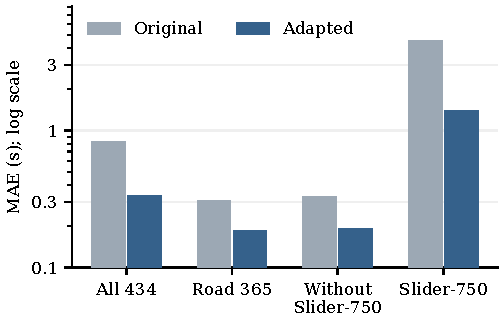
\includegraphics[width=\linewidth]{figures/adaptation.pdf}
\caption{\textbf{Exposed local adaptation.} Query-weighted EvTTC MAE before and after adaptation. The log axis makes the road and Slider populations legible. These are local comparisons from the same corrected evaluator; historical exposure prevents an independent generalization claim.}
\label{fig:adapt}
\end{figure}

\subsection{Cadence correction and promotion failure}
\EvidenceCanonicalTable
The canonical intervention preserves 2,531 road outputs and 76 of 77 Slider outputs in the frozen original fusion route, F0. Road macro MAE changes by $-0.000130406$\,s, with a descriptive 95\% interval $[-0.000504700,0.000093150]$\,s. The interval includes zero. Slider MAE decreases by 4.87\%, but this observation concerns one previously exposed recording. There are no new missing outputs or sign changes.\evid{E03}

The frozen adapted router fails the road criterion on the earlier fixed screen, despite improving aggregate metrics on the larger cohort. A paired router refit uses eight folds, three seeds, and original/canonical arms, totaling 48 fits. Its canonical ensemble improves full-population road MAE from 0.539608 to 0.537801\,s, yet worsens screen road MAE from 0.484752 to 0.511821\,s. None of the three seeds passes both views. The candidate is rejected; it does not replace the delivered adapter.\evid{E04}

On eAP, local paired replay covers all 5,805 physical queries with no new absences or sign changes. The median absolute F0 output change is approximately $14.3\,\mu$s and the maximum is 0.006496\,s. These values measure sensitivity, not accuracy: the Test12 targets remain private. The recaptured original also fails historical intermediate-state parity for all 5,805 queries and the TTC parity check for 504. Exact repeatability on the current platform does not erase this historical drift.\evid{E04}

\section{What the negative experiments establish}
\subsection{Predictive learning versus useful increments}
\EvidenceJepaTable
The bounded predictive-learning pilot uses a frozen V-JEPA~2.1 teacher~\citep{vjepa21} and 1,000 updates per arm and seed, comparing future prediction with static and shuffled-future controls. Lower future-state loss does not demonstrate a better physical representation. The expansion probe yields 0.0356400 for the candidate, 0.0376324 for the static control, and 0.0350619 for the shuffled control; neither predeclared bootstrap criterion passes. These values are MAE of dimensionless annotated log-height change, not TTC error in seconds. We retain the pilot as a negative attribution result and do not describe the final model as a demonstrated JEPA improvement.\evid{E05}

\subsection{Observability and sensor residuals}
For a linearized measurement $\mathbf y=H\boldsymbol\beta+\boldsymbol\epsilon$ and desired scalar $q=\mathbf c^\top\boldsymbol\beta$, noiseless identifiability requires $\mathbf c\perp\ker H$. This condition can hold without full rank of $H$. It is a necessary modeling distinction, but a pseudoinverse value alone does not establish reliable measurement under noise or model mismatch.

The new diagnostics separate this target-specific estimability from event support, residual magnitude, and downstream utility. Algebraic observability and a small residual do not rescue the tested normal-flow route. Robust fitting also fails to establish improvement on the exposed cohort. These findings restrict the measured route; they are not an impossibility theorem for event-based TTC.\evid{E06}

Sensor fixtures demonstrate ambiguity between motion, contrast scale, illumination, and an unknown initial event reference. A residual can fall while the inferred motion remains wrong. A physical auxiliary must therefore be evaluated on signed TTC, coverage, and appropriate nuisance controls, rather than on reconstruction alone. The inspected experiments do not justify adding their sensor residuals as calibrated confidence to the deployed fusion.\evid{E06}

\subsection{A physical clock has a restricted domain}
For positive depth $Z$, define $q=-\dot Z/Z$. Then
\begin{equation}
 \dot q=q^2-\ddot Z/Z.
\end{equation}
Under constant axial relative velocity,
\begin{equation}
 q(t+\delta)=\frac{q(t)}{1-\delta q(t)},\qquad
 T(t+\delta)=T(t)-\delta,
\label{eq:clock}
\end{equation}
provided the denominator does not cross contact. This is standard kinematics. Its composition property supplies no extra learning signal if a layer already implements the identity exactly. Acceleration, camera rotation, changing visible surfaces, and future maneuvers violate the assumptions. The tested clock and photometric extensions do not establish a better release model.\evid{E06}

\section{Runtime and numerical preservation}
\label{sec:runtime}
The runtime uses persistent modality producers, bounded causal histories, immutable input identities, and guarded cache reuse. Numerical preservation must include the actual crop, producer batch arithmetic, feature state, and final TTC. Comparing a convenient preprocessing surrogate is insufficient.

We distinguish scheduled-arrival response time, RAW-ready response time, and service span. RAW-ready begins after acquisition, copy, and sealing of the payload. Service span excludes waiting before service. Their percentiles cannot substitute for complete scheduled-arrival response time.

% Generated from evidence/runtime/summary.json.
\begin{table}[t]
\centering\small
\caption{Single-object paced replay, 250 updates. All durations are milliseconds;
the three clocks have different starting boundaries and the same complete host output endpoint.}
\label{tab:runtime}
\begin{tabular}{lrrr}
\toprule
Clock & Mean & p95 & p99 \\
\midrule
Scheduled arrival & 23.91 & 29.14 & 32.41 \\
Payload ready & 20.73 & 25.25 & 27.63 \\
Service span & 17.61 & 21.43 & 23.21 \\
\bottomrule
\end{tabular}
\end{table}

The five-second, single-object CPLA-low replay uses preloaded CPU arrivals on Windows with an NVIDIA RTX 5070 Ti Laptop GPU, FP32 arithmetic, and TF32 disabled. It excludes disk I/O and startup. It processes 250 scheduled updates with no dropped outputs or failed acknowledgments and passes the separate numerical parity check. Complete response p95 is 29.143\,ms; 201 of 250 responses reach or exceed the 20\,ms deadline. Two hundred arrivals encounter prior work. A 17.610\,ms mean service span therefore does not establish sustained deadline-compliant 50\,Hz operation.\evid{E07}

An isolated 5\,ms-prefix experiment preserves 93 ingestion boundaries, 558 persistent buffers, and eighteen TTC components exactly across three queries. It has no paced throughput result. It cannot support a 200\,Hz claim. Other crop, hash, and GPU optimizations remain isolated or fail their admission criteria; we do not combine their individual speedups into an unmeasured system speed.\evid{E07}

\section{Limitations and conclusion}
The strongest recent local improvement comes from adapting fusion over frozen measurements. It is conditional on the available object boxes, dataset history, and local evaluator. An independent generalization claim requires a new untouched cohort or an authorized official evaluation under a resolved protocol. The Slider-750 discrepancy remains open. The cadence intervention illustrates why a physically motivated correction needs downstream tests: smaller isolated errors coexist with failed fusion controls.

The uncertainty heads do not establish calibrated collision risk. In particular, an interval in inverse TTC that crosses zero maps to an unbounded or disconnected set in seconds. Saturating the output cannot remove that ambiguity. The pipeline also does not predict arbitrary future maneuvers, and the measured runtime exceeds its target deadline.

PHASE-TTC provides a causal event--RGB fusion implementation, a compact quality adapter, and reproducible positive and negative experiments. The evidence supports its archived benchmark result and its exposed local adaptation gain. It also identifies the work still needed: matched official evaluation of the adapter, independent transfer validation, reliable measurement support, and complete-output latency below the intended deadline.

\clearpage
\appendix
\section{Detection as a separate downstream diagnostic}
\label{app:detection}
The recent branches also develop an RGB 3D detector and a bridge to TTC. We include their findings to document the localization dependency, not as evidence of improved TTC. The bridge's admission panel anchors the target at exposure start and permits inference through exposure end; it therefore has a measured availability lag and is not causal at the earlier target instant. Under the aligned full-selection detection evaluator, the retained Dfull detector with a TRAIN-fitted ranker scores mAP 0.06204229, versus 0.05701726 for its baseline. Its earlier official test AP is 0.05129508 on a different population. These numbers must not share a ranking column with TTC MiD or with each other as paired test results.\evid{E08}

Range extension, class-budget changes, query ranking, KITTI transfer, and a bounded MonoCoP screen do not establish a replacement for this retained detector. Rare-class analysis and evaluation alignment explain why a seemingly promising short screen can fail on the full population. The council therefore retained detection as supporting diagnostic work.

One geometric experiment isolates a useful distinction. In an ideal target-derived cuboid test with 25,424 objects, inverting the projected cuboid edges reduces mean absolute depth error from 4.923050\,m for the height prior to approximately $2\times10^{-6}$\,m. This verifies an analytic geometry calculation with ideal inputs. On a different TRAIN diagnostic panel, substituting the corresponding estimate from predicted geometry degrades mAP from 0.21064779 to 0.16478485; a height-only substitution yields 0.08308035. Both panels contain 4,096 frames but differ in identity. The substitution also removes the learned residual, so it does not rule out retraining a compatible estimator. The analytic result is neither learned detection accuracy nor a new TTC result.\evid{E08}

\section{Additional experimental details}
\subsection{Causality and measurement availability}
Timestamp validation checks monotonic event time, exposure-time semantics, query cutoffs, and boundaries between sequences. A causal history can contain only a valid suffix if earlier observations are missing. Missing packet input, empty windows, rollback, and unavailable estimates have explicit status rather than silent zero filling. Immutable cache identity includes the admitted producer input, not merely a convenient sequence label.

The cadence intervention compares two executions on the same platform before changing elapsed-time normalization. The complete population reuses the sealed 149-query screen and extracts 2,459 additional queries. Its original control reproduces these new queries exactly within that paired experiment. This local equality and the historical eAP mismatch answer different questions and remain separate in the evidence.

\subsection{Adaptation and evaluation transformations}
The final router fit excludes the competition recordings from optimizer updates, but model choices inherit earlier exposure. We distinguish this final fit exclusion from a pristine evaluation split. The three router seeds share all upstream components and cannot quantify representation uncertainty. The delivered adapter also preserves signed negative predictions; the organizer-style interpolation belongs only to the documented local scoring comparison.

The corrected 434-row analysis supersedes earlier 423-row summaries. We do not discard the eleven recovered targets or modify timestamps to align a score. We preserve the official-versus-local Slider-750 discrepancy rather than changing the error reduction to reproduce the reported value. All subsets in the adaptation table use query-weighted reductions. The canonical table instead reports recording-macro means and availability denominators.

\subsection{Physical and predictive controls}
The sensor tests distinguish complete observed silence from missing or filtered events. Without a known or marginalized initial sensor reference, the absence of threshold crossings does not imply a particular motion. When illumination or threshold parameters can absorb any residual, a reconstruction objective cannot identify expansion on its own.

The JEPA controls preserve a future marginal while breaking correspondence, so an improvement over a static representation is insufficient if shuffled futures perform as well. Small physical increments require a downstream readout under the declared grouping and bootstrap. This motivates retaining the failed control comparison even though the predictive objective decreased.

\section{Evidence and reproducibility}
\label{app:evidence}
This revision preserves the earlier manuscript and adds a separate source tree. We reviewed local and fetched remote branch histories for the five-day lookback beginning 28 October 2026, including work on 2 November. The review manifest records the exact cutoff, refs, commits, Markdown paths, and content hashes. Council reports cover fusion/transfer, runtime, detection, reference style, and the remaining physics/documentation work. Their inclusion decisions accompany the article; they are editorial judgments, not independent experimental replications.

The source package contains a deterministic evidence-table generator, copied source ledgers where needed, SHA-256 manifests, the LaTeX source, and the PDF build script. Rebuilding tables and figures uses saved results, not model training or private Test12 labels. A structured registry maps the evidence identifiers below to paths and pinned refs. Paths in Git refer to their recorded revision rather than an assumed current default branch.

\begin{description}
\item[E01] Original TRAIN40 architecture and grouped fitting: the preceding paper's method sources; official scores: \texttt{paper/data/official\_benchmark.json}, snapshot 28 October 2026.
\item[E02] Adapted model and corrected 434-query evaluator: \texttt{docs/research\_progress\_20261101} and the sign-safe evaluator audit. Includes historical exposure and the unresolved Slider-750 row.
\item[E03] Canonical PAIR, complete development population: \texttt{docs/research\_log\_canonical\_population2608}; paired predictions, recording metrics, and bootstrap.
\item[E04] Native eAP recapture and rejected paired refit: \texttt{docs/research\_progress\_20261101/v1/evidence}.
\item[E05] Closed predictive-learning pilot: audited future-prediction and physical-increment probes. The evidence table generator records the exact source keys.
\item[E06] Physics review and completed follow-ups: \texttt{docs/physics\_review\_20261031} and \texttt{docs/release\_research\_implementation\_20261031}.
\item[E07] Paced runtime summary and council archive dated 28 October 2026; successful-output latency population, parity results, and isolated prefix test.
\item[E08] Detection branch diagnostics through 2 November 2026; copied ledgers retain their original branch and commit identities.
\end{description}

\subsection{Visual design provenance}
We independently reproduce the typographic layout inspected in the supplied \texttt{arXiv-2608.27395v1.tar.gz}: US Letter, two columns, Latin Modern at 9.3\,pt, 0.72-inch side margins, a full-width pale-blue abstract, booktabs tables, numeric citations, and centered folios. The archive's main file overrides its theme by disabling running headers. We retain that effective layout. Scientific text, authorship, figures, and numerical examples from the reference are not reused.

\newpage
\bibliographystyle{plainnat}
\bibliography{references}
\end{document}
